\chapter[The \index{tychonoff theorem@Tychonoff theorem}\index{tychonoff theorem@Tychonoff theorem}Tychonoff Theorem]{The Tychonoff Theorem}
\vspace{6.5cm}
\chaptermark{The Tychonoff Theorem}


We now return to a problem we left unresolved in Chapter 3. We shall prove the \index{Tychonoff theorem}, to the effect that arbitrary products of compact spaces are compact. The proof makes use of Zorn's Lemma (see §11). An alternate proof, which relies instead on the well-ordering theorem, is outlined in the exercises.

The \index{Tychonoff theorem}\index{Tychonoff theorem}Tychonoff theorem is of great usefulness to analysts (less so to geometers). We apply it in §38 to construct the Stone-Čech compactification of a completely regular space, and in \(\$ {47}\) in proving the general version of Ascoli's theorem.

\section*{§ 37 The Tychonoff Theorem}

Like the Urysohn lemma, the Tychonoff theorem is what we call a ``deep'' theorem. Its proof involves not one but several original ideas; it is anything but straightforward. We shall discuss the crucial ideas of the proof in some detail before turning to the proof itself.

In Chapter 3, we proved the product \(X \times  Y\) of two compact spaces to be compact. For that proof the open covering formulation of compactness was quite satisfactory. Given an open covering of \(X \times  Y\) by basis elements, we covered each slice \(x \times  Y\) by finitely many of them, and proceeded from that to construct a finite covering of \(X \times  Y\) .

It is quite tricky to make this approach work for an arbitrary product of compact spaces; one must well-order the index set and use transfinite induction. (See Exercise 5.) An alternate approach is to abandon open coverings and to approach the problem by applying the closed set formulation of compactness, using Zorn's lemma.

To see how this idea might work, let us consider first the simplest possible case: the product of two compact spaces \({X}_{1} \times  {X}_{2}\) . Suppose that \(\mathcal{A}\) is a collection of closed subsets of \({X}_{1} \times  {X}_{2}\) that has the finite intersection property. Consider the projection map \({\pi }_{1} : {X}_{1} \times  {X}_{2} \rightarrow  {X}_{1}\) . The collection

\[
\{  {{\pi }_{1}( A)  \mid  A \in  \mathcal{A}}\}
\]

of subsets of \({X}_{1}\) also has the finite intersection property, and so does the collection of their closures \(\overline{{\pi }_{1}( A) }\) . Compactness of \({X}_{1}\) guarantees that the intersection of all the sets \(\overline{{\pi }_{1}( A) }\) is nonempty. Let us choose a point \({x}_{1}\) belongingg to this intersection. Similarly, let us choose a point \({x}_{2}\) belongingg to all the sets \(\overline{{\pi }_{2}( A) }\) . The obvious conclusion we would like to draw is that the point \({x}_{1} \times  {x}_{2}\) lies in \(\mathop{\bigcap }\limits_{{A \in  A}}A\) , for then our theorem would be proved.

But that is unfortunately not true. Consider the following example, in which \({X}_{1} =\)  \({X}_{2} = [  {0,1}]\) and the collection \(\mathcal{A}\) consists of all closed elliptical regions bounded by ellipses that have the points \(p = ( {\frac{1}{3},\frac{1}{3}})\) and \(q = ( {\frac{1}{2},\frac{2}{3}})\) as their foci. See Figure 37.1. Certainly \(\mathcal{A}\) has the finite intersection property. Now let us pick a point \({x}_{1}\) in the intersection of the sets \(\{  {. \overline{{\pi }_{1}( A) }| \;A \in  \mathcal{A}}\}\) Any point of the interval \([  {\frac{1}{3},\frac{1}{2}}]\) will do; suppose we choose \({x}_{1} = \frac{1}{2}\) . Similarly, choose a point \({x}_{2}\) in the intersection of the sets \(\{  {\overline{{\pi }_{2}( A) } \mid  A \in  \mathcal{A}}\}\) . Any point of the interval \([  {\frac{1}{3},\frac{2}{3}}]\) will do; suppose we pick \({x}_{2} = \frac{1}{2}\) . This proves to be an unfortunate choice, for the point

\[
{x}_{1} \times  {x}_{2} = \frac{1}{2} \times  \frac{1}{2}
\]

does not lie in the intersection of the sets \(A\) .

\begin{center}
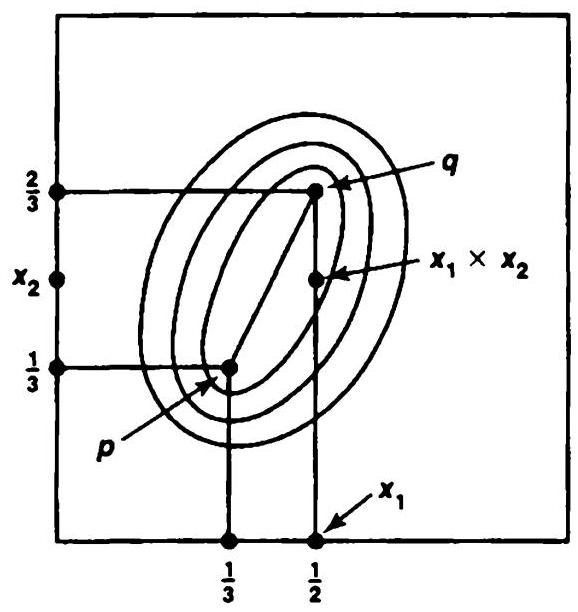
\includegraphics[width=0.5\textwidth]{images/37.1.jpg}
\end{center}
\hspace*{3em} 

Figure 37.1

``Aha!'' you say,''you made a bad choice. If after choosing \({x}_{1} = \frac{1}{2}\) you had chosen \({x}_{2} = \frac{2}{3}\) , then you would have found a point in \(\mathop{\bigcap }\limits_{{A \in  \mathcal{A}}}A\) .'' The difficulty with our tentative proof is that it gave us too much freedom in picking \({x}_{1}\) and \({x}_{2}\) ; it allowed us to make a ``bad'' choice instead of a ``good'' choice.

How can we alter the proof so as to avoid this difficulty?

This question leads to the second idea of the proof: Perhaps if we expand the collection \(\mathcal{A}\) (retaining the finite intersection property, of course), that expansion will restrict the choices of \({x}_{1}\) and \({x}_{2}\) sufficiently that we will be forced to make the ``right'' choice. To illustrate, suppose that in the previous example we expand the collection \(\mathcal{A}\) to the collection \(\mathcal{D}\) consisting of all closed elliptical regions bounded by ellipses that have \(p = ( {\frac{1}{3},\frac{1}{3}})\) as one focus and any point of the line segment \({pq}\) as the other focus. This collection is illustrated in Figure 37.2. The new collection \(\mathcal{D}\) still has the finite intersection property. But if you try to choose a point \({x}_{1}\) in

\[
\mathop{\bigcap }\limits_{{D \in  \mathcal{D}}}\overline{{\pi }_{1}( D) }
\]

the only possible choice for \({x}_{1}\) is \(\frac{1}{3}\) Similarly, the only possible choice for \({x}_{2}\) is \(\frac{1}{3}\) . And \(\frac{1}{3} \times  \frac{1}{3}\) does belong to every set \(D\) , and hence to every set \(A\) . In other words, expanding the collection \(\mathcal{A}\) to the collection \(\mathcal{D}\) forces the proper choice on us.

\begin{center}
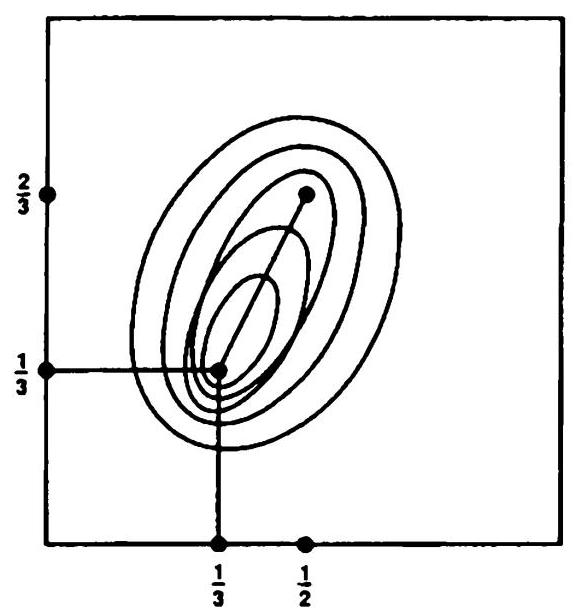
\includegraphics[width=0.5\textwidth]{images/37.2.jpg}
\end{center}
\hspace*{3em} 

Figure 37.2

Now of course in this example we chose \(\mathcal{D}\) carefully so that the proof would work. What hope can we have for choosing \(\mathcal{D}\) correctly in general? Here is the third idea of the proof: Why not simply choose \(\mathcal{D}\) to be a collection that is ``as large as possible''- so that no larger collection has the finite intersection property—and see whether such a \(\mathcal{D}\) will work? It is not at all obvious that such a collection \(\mathcal{D}\) exists; to prove it, we must appeal to Zorn's lemma. But after we prove that \(\mathcal{D}\) exists, we shall in fact be able to show that \(\mathcal{D}\) is large enough to force the proper choices on us.

A final remark. The assumption that the elements of the collection \(\mathcal{A}\) were closed sets was irrelevant in this discussion. For even if the set \(A \in  \mathcal{A}\) is closed, the set \({\pi }_{1}( A)\) need not be closed, so we had to take its closure in order to apply the closed set formulation of compactness. Therefore, we may as well begin with an arbitrary collection of subsets of \(X\) having the finite intersection property, and prove that the intersection of their closures is nonempty. This approach actually proves to be more convenient.

\begin{lemma}
	Let \(X\) be a set; let \(\mathcal{A}\) be a collection of subsets of \(X\) having the finite intersection property. Then there is a collection \(\mathcal{D}\) of subsets of \(X\) such that \(\mathcal{D}\) contains \(\mathcal{A}\) , and \(\mathcal{D}\) has the finite intersection property, and no collection of subsets of \(X\) that properly contains \(\mathcal{D}\) has this property.
\end{lemma}

We often say that a collection \(\mathcal{D}\) satisfying the conclusion of this theorem is maximal with respect to the finite intersection property

\begin{proof}
	As you might expect, we construct \(\mathcal{D}\) by using Zorn's lemma. It states that, given a set \(A\) that is strictly partially ordered, in which every simply ordered subset has an upper bound, \(A\) itself has a maximal element.
The set \(A\) to which we shall apply Zorn's lemma is not a subset of \(X\) , nor even a collection of subsets of \(X\) , but a set whose elements are collections of subsets of \(X\) . For purposes of this proof, we shall call a set whose elements are collections of subsets of \(X\) a ``\index{superset}'' and shall denote it by an outline letter. To summarize the rotation:

\(c\) is an element of \(X\) .

\(C\) is a subset of \(X\)

\(C\) is a collection of subsets of \(X\)

\(\mathbb{C}\) is a \index{Superset}\index{Superset}\index{superset@Superset}\index{superset@Superset}superset whose elements are collections of subsets of \(X\) .

Now by hypothesis, we have a collection \(\mathcal{A}\) of subsets of \(X\) that has the finite intersection property. Let \(\mathbf{A}\) denote the superset consisting of all collections \(\mathcal{B}\) of subsets of \(X\) such that \(\mathcal{B} \supset  \mathcal{A}\) and \(\mathcal{B}\) has the finite intersection property. We use proper inclusion \(\subsetneq\) as our strict partial order on \(\mathbf{A}\) . To prove our lemma, we need to show that \(\mathbf{A}\) has a maximal element \(\mathcal{D}\) .

In order to apply Zorn's lemma, we must show that if \(\mathbb{B}\) is a ``subsuperset'' of \(\mathbf{A}\) that is simply ordered by proper inclusion, then \(\mathbb{B}\) has an upper bound in \(\mathbb{A}\) . We shall show in fact that the collection

\[
\mathcal{C} = \mathop{\bigcup }\limits_{{\mathcal{B} \in  \mathbb{B}}}\mathcal{B}
\]

which is the union of the collections belongingg to \(\mathbb{B}\) , is an element of \(\mathbb{A}\) , then it is the required upper bound on \(\mathbb{B}\) .

To show that \(\mathcal{C}\) is an element of \(\mathbf{A}\) , we must show that \(\mathcal{C} \supset  \mathcal{A}\) and that \(\mathcal{C}\) has the finite intersection property. Certainly \(\mathcal{C}\) contains \(\mathcal{A}\) , since each element of \(\mathcal{B}\) contains \(\mathcal{A}\) . To show that \(\mathcal{C}\) has the finite intersection property, let \({C}_{1},\ldots ,{C}_{n}\) be elements, of \(\mathcal{C}\) . Because \(\mathcal{C}\) is the union of the elements of \(\mathbb{B}\) , there is, for each \(i\) , an element \({\mathcal{B}}_{i}\) of \(\mathbb{B}\) such that \({C}_{i} \in  {\mathcal{B}}_{i}\) . The superset \(\{  {{\mathcal{B}}_{1},\ldots ,{\mathcal{B}}_{n}}\}\) is contained in \(\mathbb{B}\) , so it is simply ordered by the relation of proper inclusion. Being finite, it has a largest element; that is, there is an index \(k\) such that \({\mathcal{B}}_{i} \subset  {\mathcal{B}}_{k}\) for \(i = 1,\ldots ,n\) . Then all the sets \({C}_{1},\ldots ,{C}_{n}\) are elements of \({\mathcal{B}}_{k}\) . Since \({\mathcal{B}}_{k}\) has the finite intersection property, the intersection of the sets \({C}_{1},\ldots ,{C}_{n}\) is nonempty, as desired.
\end{proof}
\begin{lemma}
	Let \(X\) be a set; let \(\mathcal{D}\) be a collection of subsets of \(X\) that is maximal with respect to the finite intersection property. Then:

(a) Any finite intersection of elements of \(\mathcal{D}\) is an element of \(\mathcal{D}\) .

(b) If \(A\) is a subset of \(X\) that intersects every element of \(\mathcal{D}\) , then \(A\) is an element of \(\mathcal{D}\) .
\end{lemma}

\begin{proof}
	(a) Let \(B\) equal the intersection of finitely many elements of \(\mathcal{D}\) . Define a collection \(\mathcal{E}\) by adjoining \(B\) to \(\mathcal{D}\) , so that \(\mathcal{E} = \mathcal{D} \cup  \{ B\}\) . We show that \(\mathcal{E}\) has the finite intersection property; then maximality of \(\mathcal{D}\) implies that \(\mathcal{E} = \mathcal{D}\) , so that \(B \in  \mathcal{D}\) as desired
Take finitely many elements of \(\mathcal{E}\) . If none of them is the set \(B\) , then their intersection is nonempty because \(\mathcal{D}\) has the finite intersection property. If one of them is the set \(B\) , then their intersection is of the form

\[
{D}_{1} \cap   \cdot   \cdot   \cap  {D}_{m} \cap  B
\]

Since \(B\) equals a finite intersection of elements of \(\mathcal{D}\) , this set is nonempty.

(b) Given \(A\) , define \(\mathcal{E} = \mathcal{D} \cup  \{ A\}\) We show that \(\mathcal{E}\) has the finite intersection property, from which we conclude that \(A\) belongs to \(\mathcal{D}\) . Take finitely many elements of \(\mathcal{E}\) . If none of them is the set \(A\) , their intersection is automatically nonempty. Otherwise, it is of the form

\[
{D}_{1} \cap  \cdots  \cap  {D}_{n} \cap  A\text{ . }
\]

Now \({D}_{1} \cap  \cdots  \cap  {D}_{n}\) belongs to \(\mathcal{D}\) , by (a); therefore, this intersection is nonempty, by hypothesis.
\end{proof}
\begin{theorem}[Tychon\index{Compactness!of product space}\index{Compactness!of product space}off theorem]
	An arbitrary product of compact spaces is compact in the product topology
\end{theorem}

\begin{proof}
	Let
\[
X = \mathop{\prod }\limits_{{\alpha  \in  J}}{X}_{\alpha }
\]

where each space \({X}_{\alpha }\) is compact. Let \(\mathcal{A}\) be a collection of subsets of \(X\) having the finite intersection property. We prove that the intersection

\[
\mathop{\bigcap }\limits_{{A \in  A}}\bar{A}
\]

is nonempty. Compactness of \(X\) follows.

Applying Lemma 37.1, choose a collection \(\mathcal{D}\) of subsets of \(X\) such that \(\mathcal{D} \supset  \mathcal{A}\) and \(\mathcal{D}\) is maximal with respect to the finite intersection property It will suffice to show that the intersection \(\mathop{\bigcap }\limits_{{D \in  \mathcal{D}}}\bar{D}\) is nonempty.

Given \(\alpha  \in  J\) , let \({\pi }_{\alpha } : X \rightarrow  {X}_{\alpha }\) be the projection map, as usual Consider the collection

\[
\{  {{\pi }_{\alpha }( D)  \mid  D \in  \mathcal{D}}\}
\]

of subsets of \({X}_{\alpha }\) . This collection has the finite intersection property because \(\mathcal{D}\) does. By compactness of \({X}_{\alpha }\) , we can for each \(\alpha\) choose a point \({x}_{\alpha }\) of \({X}_{\alpha }\) such that

\[
{x}_{\alpha } \in  \mathop{\bigcap }\limits_{{D \in  \mathcal{D}}}\overline{{\pi }_{\alpha }( D) }.
\]

Let \(\mathbf{x}\) be the point \({( {x}_{\alpha }) }_{\alpha  \in  J}\) of \(X\) . We shall show that \(\mathbf{x} \in  \bar{D}\) for every \(D \in  \mathcal{D}\) ; then our proof will be finished.

First we show that if \({\pi }_{\beta }^{-1}( {U}_{\beta })\) is any subbasis element (for the product topology on \(X\) ) containing \(\mathbf{x}\) , then \({\pi }_{\beta }^{-1}( {U}_{\beta })\) intersects every element of \(\mathcal{D}\) . The set \({U}_{\beta }\) is a neighborhood of \({x}_{\beta }\) in \({X}_{\beta }\) . Since \({x}_{\beta } \in  \overline{{\pi }_{\beta }( D) }\) by definition, \({U}_{\beta }\) intersects \({\pi }_{\beta }( D)\) in some point \({\pi }_{\beta }( \mathbf{y})\) , where \(\mathbf{y} \in  D\) Then it follows that \(\mathbf{y} \in  {\pi }_{\beta }^{-1}( {U}_{\beta })  \cap  D\) .

It follows from (b) of Lemma 37.2 that every subbasis element containing \(\mathbf{x}\) belongs to \(\mathcal{D}\) . And then it follows from (a) of the same lemma that every basis element containing \(\mathbf{x}\) belongs to \(\mathcal{D}\) . Since \(\mathcal{D}\) has the finite intersection property, this means that every basis element containing \(\mathbf{x}\) intersects every element of \(\mathcal{D}\) ; hence \(\mathbf{x} \in  \bar{D}\) for every \(D \in  \mathcal{D}\) as desired.
\end{proof}
\section*{Exercises}
\begin{enumerate}[itemsep=0.4em, parsep=0pt, topsep=0pt, partopsep=0pt, leftmargin=*, label=\arabic*., ref=\arabic*]
\item Let \(X\) be a space. Let \(\mathcal{D}\) be a collection of subsets of \(X\) that is maximal with respect to the finite intersection property
  \begin{enumerate}[itemsep=0.2em, parsep=0pt, topsep=0pt, partopsep=0pt, leftmargin=*, label=(\alph*), align=left]
  \item Show that \(x \in  \bar{D}\) for every \(D \in  \mathcal{D}\) if and only if every neighborhood of \(x\) belongs to \(\mathcal{D}\) . Which implication uses maximality of \(\mathcal{D}\) ?
  \item Let \(D \in  \mathcal{D}\) . Show that if \(A \supset  D\) , then \(A \in  \mathcal{D}\) .
  \item Show that if \(X\) satisfies the \({T}_{1}\) axiom, there is at most one point belongingg to \(\mathop{\bigcap }\limits_{{D \in  \mathcal{D}}}\bar{D}\) .
  \end{enumerate}
\item A collection \(\mathcal{A}\) of subsets of \(X\) has the \index{countable intersection property} if every countable intersection of elements of \(\mathcal{A}\) is nonempty. Show that \(X\) is a Lindelöf space if and only if for every collection \(\mathcal{A}\) of subsets of \(X\) having the \index{Countable intersection property}\index{Countable intersection property}\index{countable intersection property@Countable intersection property}\index{countable intersection property@Countable intersection property}countable intersection property,
\end{enumerate}
\section*{\(\mathop{\bigcap }\limits_{{A \in  A}}\bar{A}\)}

is nonempty.

3. Consider the three statements:

(i) If \(X\) is a set and \(\mathcal{A}\) is a collection of subsets of \(X\) having the countable intersection property, then there is a collection \(\mathcal{D}\) of subsets of \(X\) such that \(\mathcal{D} \supset  \mathcal{A}\) and \(\mathcal{D}\) is maximal with respect to the countable intersection property

(ii) Suppose \(\mathcal{D}\) is maximal with respect to the countable intersection property Then countable intersections of elements of \(\mathcal{D}\) are in \(\mathcal{D}\) . Furthermore, if \(A\) is a subset of \(X\) that intersects every element of \(\mathcal{D}\) , then \(A\) is an element of \(\mathcal{D}\) .

(iii) Products of Lindelöf spaces are Lindelöf.

(a) Show that (i) and (ii) together imply (iii).

(b) Show that (ii) holds.

(c) Products of Lindelöf spaces need not be Lindelöf (see §30). Therefore (i) does not hold. If one attempts to generalize the proof of Lemma 37.1 to the countable intersection property, at what point does the proof break down?

4. Here is another theorem whose proof uses Zorn's lemma. Recall that if \(A\) is a space and if \(x,y \in  A\) , we say that \(x\) and \(y\) belong to the same quasicomponent of \(A\) if there is no separation \(A = C \cup  D\) of \(A\) into two disjoint sets open in \(A\) such that \(x \in  C\) and \(y \in  D\) .

\begin{theorem}
	Let \(X\) be a compact Hausdorff space. Then \(x\) and \(y\) belong to the same quasicomponent of \(X\) if and only if they belong to the same component of \(X\) .
\end{theorem}

(a) Let \(A\) be the collection of all closed subspaces \(A\) of \(X\) such that \(x\) and \(y\) lie in the same quasicomponent of \(A\) . Let \(\mathcal{B}\) be a subcollection of \(\mathcal{A}\) that is simply ordered by proper inclusion. Show that the intersection of the elements of \(\mathcal{B}\) belongs to \(\mathcal{A}\) . [Hint: Compare Exercise 11 of §26.]

(b) Show \(\mathcal{A}\) has a minimal element \(D\) .

(c) Show \(D\) is connected.

*5. Here is a proof of the Tychonoff theorem that relies on the well-ordering theorem rather than on Zorn's lemma. First, prove the following version of the tube lemma; then prove the theorem.

\begin{lemma}
	Let \(\mathcal{A}\) be a collection of basis elements for the topology of the product space \(X \times  Y\) , such that no finite subcollection of \(\mathcal{A}\) covers \(X \times  Y\) . If \(X\) is compact, there is a point \(x \in  X\) such that no finite subcollection of \(\mathcal{A}\) covers the slice \(\{ x\}  \times  Y\) .
\end{lemma}

\begin{theorem}
	An arbitrary product of compact spaces is compact in the product topology.
\end{theorem}

\begin{proof}
	Let \({\{  {X}_{\alpha }\}  }_{\alpha  \in  J}\) be an indexed family of compact spaces, let
\[
X = \mathop{\prod }\limits_{{\alpha  \in  J}}{X}_{\alpha }
\]

Let \({\pi }_{\alpha } : X \rightarrow  {X}_{\alpha }\) be the projection map. Well-order \(J\) , once and for all, in such a way that \(J\) has a largest element.

(a) Let \(\beta  \in  J\) Suppose points \({p}_{i} \in  {X}_{i}\) are given, for all \(i < \beta\) . For any \(\alpha  < \beta\) , let \({Y}_{\alpha }\) denote the subspace of \(X\) defined by the equation

\[
{Y}_{\alpha } = \{  {\mathbf{x} \mid  {\pi }_{i}( \mathbf{x})  = {p}_{i}\text{ for }i \leq  \alpha }\}  .
\]

Note that if \(\alpha  < {\alpha }^{\prime }\) , then \({Y}_{\alpha } \supset  {Y}_{{\alpha }^{\prime }}\) . Show that if \(\mathcal{A}\) is a finite collection of

basis elements for \(X\) that covers the space

\[
{Z}_{\beta } = \mathop{\bigcap }\limits_{{\alpha  < \beta }}{Y}_{\alpha } = \{  {\mathbf{x} \mid  {\pi }_{i}( \mathbf{x})  = {p}_{i}\text{ for }i < \beta }\}
\]

then \(\mathcal{A}\) actually covers \({Y}_{\alpha }\) for some \(\alpha  < \beta\) . [Hint. If \(\beta\) has an immediate predecessor in \(J\) , let \(\alpha\) be that immediate predecessor Otherwise, for each \(A \in  \mathcal{A}\) , let \({J}_{A}\) denote the set of those indices \(i < \beta\) for which \({\pi }_{i}( A)  \neq  {X}_{i}\) ; the union of the sets \({J}_{A}\) , for \(A \in  \mathcal{A}\) , is finite; let \(\alpha\) be the largest element of this union.]

(b) Assume \(\mathcal{A}\) is a collection of basis elements for \(X\) such that no finite subcol-lection of \(\mathcal{A}\) covers \(X\) . Show that one can choose points \({p}_{i} \in  {X}_{i}\) for all \(i\) , such that for each \(\alpha\) , the space \({Y}_{\alpha }\) defined in (a) cannot be finitely covered by \(\mathcal{A}\) . When \(\alpha\) is the largest element of \(J\) , one has a contradiction. [Hint: If \(\alpha\) is the smallest element of \(J\) , use the preceding lemma to choose \({p}_{\alpha }\) . If \({p}_{i}\) is defined for all \(i < \beta\) , note that (a) implies that the space \({Z}_{\beta }\) cannot be finitely covered by \(\mathcal{A}\) and use the lemma to find \({p}_{\beta }\) ]
\end{proof}
\section*{§ 38 The Stone-Čech Compactification}

We have already studied one way of compactifying a topological space \(X\) , the one-point compactification (§29); it is in some sense the minimal compactification of \(X\) . The Stone-Čech compactification of \(X\) , which we study now, is in some sense the maximal compactification of \(X\) . It was constructed by M. Stone and E. Čech, independently, in 1937 It has a number of applications in modern analysis, but these lie outside the scope of this book

We recall the following definition

\begin{definition}
	A compactification of a space \(X\) is a compact Hausdorff space \(Y\) containing \(X\) as a subspace such that \(\bar{X} = Y\) . Two compactifications \({Y}_{1}\) and \({Y}_{2}\) of \(X\) are said to be equivalent if there is a homeomorphism \(h : {Y}_{1} \rightarrow  {Y}_{2}\) such that \(h( x)  = x\) for every \(x \in  X\) .
\end{definition}

If \(X\) has a compactification \(Y\) , then \(X\) must be completely regular, being a subspace of the completely regular space \(Y\) . Conversely, if \(X\) is completely regular, then \(X\) has a compactification. For \(X\) can be imbedded in the compact Hausdorff space \({[  0,1]  }^{J}\) for some \(J\) , and any such imbedding gives rise to a compactification of \(X\) , as the following lemma shows

\begin{lemma}
	Let \(X\) be a space; suppose that \(h : X \rightarrow  Z\) is an imbedding of \(X\) in the compact Hausdorff space \(Z\) . Then there exists a corresponding compactification \(Y\) of \(X\) ; it has the property that there is an imbedding \(H : Y \rightarrow  Z\) that equals \(h\) on \(X\) . The compactification \(Y\) is uniquely determined up to \index{Equivalence of compactifications} equivalence.
\end{lemma}

We call \(Y\) the compactification induced by the imbedding \(h\) .

\begin{proof}
	Given \(h\) , let \({X}_{0}\) denote the subspace \(h( X)\) of \(Z\) , and let \({Y}_{0}\) denote its closure in \(Z\) . Then \({Y}_{0}\) is a compact Hausdorff space and \({\bar{X}}_{0} = {Y}_{0}\) ; therefore, \({Y}_{0}\) is a compactification of \({X}_{0}\) .
We now construct a space \(Y\) containing \(X\) such that the pair(X, Y)is homeomorphic to the pair \(( {{X}_{0},{Y}_{0}})\) . Let us choose a set \(A\) disjoint from \(X\) that is in bijective correspondence with the set \({Y}_{0} - {X}_{0}\) under some map \(k : A \rightarrow  {Y}_{0} - {X}_{0}\) . Define \(Y = X \cup  A\) , and define a bijective correspondence \(H : Y \rightarrow  {Y}_{0}\) by the rule

\[
H( x)  = h( x) \;\text{ for }x \in  X,
\]

\[
H( a)  = k( a) \;\text{ for }a \in  A.
\]

Then topologize \(Y\) by declaring \(U\) to be open in \(Y\) if and only if \(H( U)\) is open in \({Y}_{0}\) . The map \(H\) is automatically a homeomorphism; and the space \(X\) is a subspace of \(Y\) because \(H\) equals the homeomorphism \(h\) when restricted to the subspace \(X\) of \(Y\) . By expanding the range of \(H\) , we obtain the required imbedding of \(Y\) into \(Z\) .

Now suppose \({Y}_{i}\) is a compactification of \(X\) and that \({H}_{i} : {Y}_{i} \rightarrow  Z\) is an imbedding that is an extension of \(h\) , for \(i = 1,2\) . Now \({H}_{i}\) maps \(X\) onto \(h( X)  = {X}_{0}\) Because \({H}_{t}\) is continuous, it must map \({Y}_{t}\) into \({\bar{X}}_{0}\) ; because \({H}_{i}( {Y}_{i})\) contains \({X}_{0}\) and is closed (being compact), it contains \({\bar{X}}_{0}\) . Hence \({H}_{i}( {Y}_{i})  = {\bar{X}}_{0}\) , and \({H}_{2}^{-1} \circ  {H}_{1}\) defines a homeomorphism of \({Y}_{1}\) with \({Y}_{2}\) that equals the identity on \(X\) .

In general, there are many different ways of compactifying a given space \(X\) . Consider for instance the following compactifications of the open interval \(X = ( {0,1})\) :

\begin{centeredblock}
\begin{example}
	Take the unit circle \({S}^{1}\) in \({\mathbb{R}}^{2}\) and let \(h.( {0,1})  \rightarrow  {S}^{1}\) be the map

\[
h( \iota )  = ( {\cos {2\pi \iota }})  \times  ( {\sin {2\pi \iota }}) .
\]

The compactification induced by the imbedding \(h\) is equivalent to the one-point compactification of \(X\)
\end{example}
\end{centeredblock}

\begin{centeredblock}
\begin{example}
	Let \(Y\) be the space \([  {0,1}]\) Then \(Y\) is a compacufication of \(X\) , it is obtained by ``adding one point at each end of(0,1)''
\end{example}
\end{centeredblock}

\begin{centeredblock}
\begin{example}
	Consider the square \({[  -1,1]  }^{2}\) in \({\mathbb{R}}^{2}\) and let \(h\;( {0,1})  \rightarrow  {[  -1,1]  }^{2}\) be the map

\[
h( x)  = x \times  \sin ( {1/x}) .
\]

The space \({Y}_{0} = \overline{h( X) }\) is the topologist's sine curve (see Example 7 of §24). The imbedding \(h\) gives rise to a compactification of(0,1)quite different from the other two. It is obtained by adding one point at the right-hand end of(0,1), and an entire line segment of points at the left-hand end \({}^{1}\)
\end{example}
\end{centeredblock}

A basic problem that occurs in studying compactifications is the following:

If \(Y\) is a compactification of \(X\) , under what conditions can a continuous real-valued function \(f\) defined on \(X\) be extended continuously to \(Y\) ? The function \(f\) will have to be bounded if it is to be extendable, since its extension will carry the compact space \(Y\) into \(\mathbb{R}\) and will thus be bounded. But boundedness is not enough, in general. Consider the following example

\begin{centeredblock}
\begin{example}
	Let \(X = ( {0,1})\) Consider the one-point compactification of \(X\) given in Example I A bounded continuous function \(f : ( {0,1})  \rightarrow  \mathbb{R}\) is extendable to this compacutfication if and only if the limits

\[
\mathop{\lim }\limits_{{x \rightarrow  0 + }}f( x) \;\text{ and }\;\mathop{\lim }\limits_{{x \rightarrow  1 - }}f( x)
\]

exist and are equal.
\end{example}
\end{centeredblock}

For the ``the two-point compactification'' of \(X\) considered in Example 2, the function \(f\) is extendable if and only if both these limits simply exist

For the compactification of Example 3, extensions exist for a still broader class of functions It is easy to see that \(f\) is extendable if both the above limits exist But the function \(f( x)  = \sin ( {1/x})\) is also extendable to this compactification. Let \(H\) be the imbedding of \(Y\) in \({\mathbb{R}}^{2}\) that equals \(h\) on the subspace \(X\) Then the composite map

\[
Y\overset{H}{ \rightarrow  }\mathbb{R} \times  \mathbb{R}\overset{{\pi }_{2}}{ \rightarrow  }\mathbb{R}
\]

is the desired extension of \(f\) . For if \(x \in  X\) , then \(H( x)  = h( x)  = x \times  \sin ( {1/x})\) , so that \({\pi }_{2}( {H( x) })  = \sin ( {1/x})\) , as desired

There is something especially interesting about this last compactification. We constructed it by choosing an imbedding

\[
h.( {0,1})  \rightarrow  {\mathbb{R}}^{2}
\]

whose component functions were the functions \(x\) and \(\sin ( {1/x})\) Then we found that both the functions \(x\) and \(\sin ( {1/x})\) could be extended to the compactification This suggests that if we have a whole collection of bounded continuous functions defined on(0,1), we might use them as component functions of an imbedding of(0,1)into \({\mathbb{R}}^{J}\) for some \(J\) , and thereby obtain a compactification for which every function in the collection is extendable.

This idea is the basic idea behind the Stone-Čech compactification. It is defined as follows:
\end{proof}
\begin{theorem}
	Let \(X\) be a completely regular space. There exists a compactification \(Y\) of \(X\) having the property that every bounded continuous map \(f : X \rightarrow  \mathbb{R}\) extends uniquely to a continuous map of \(Y\) into \(\mathbb{R}\) .
\end{theorem}

\begin{proof}
	Let \({\{  {f}_{\alpha }\}  }_{\alpha  \in  J}\) be the collection of all bounded continuous real-valued functions on \(X\) , indexed by some index set \(J\) For each \(\alpha  \in  J\) , choose a closed interval \({I}_{\alpha }\) in \(\mathbb{R}\) containing \({f}_{\alpha }( X)\) . To be definite, choose
\[
{I}_{\alpha } = \{  {\inf {f}_{\alpha }( X) ,\sup {f}_{\alpha }( X) }\}  .
\]

Then define \(h : X \rightarrow  \mathop{\prod }\limits_{{\alpha  \in  J}}{I}_{\alpha }\) by the rule

\[
h( x)  = {( {f}_{\alpha }( x) ) }_{\alpha  \in  J}.
\]

By the Tychonoff theorem, \(\prod {I}_{\alpha }\) is compact Because \(X\) is completely regular, the collection \(\{  {f}_{\alpha }\}\) separates points from closed sets in \(X\) . Therefore, by Theorem 34.2, the map \(h\) is an imbedding.

Let \(Y\) be the compactification of \(X\) \index{Compactification!induced by an imbedding}\index{Compactification!induced by an imbedding}induced by the imbedding \(h\) . Then there is an imbedding \(H : Y \rightarrow  \prod {I}_{\alpha }\) that equals \(h\) when restricted to the subspace \(X\) of \(Y\) . Given a bounded continuous real-valued function \(f\) on \(X\) , we show it extends to \(Y\) . The function \(f\) belongs to the collection \({\{  {f}_{\alpha }\}  }_{\alpha  \in  J}\) , so it equals \({f}_{\beta }\) for some index \(\beta\) . Let \({\pi }_{\beta }.\prod {I}_{\alpha } \rightarrow  {I}_{\beta }\) be the projection mapping Then the continuous map \({\pi }_{\beta } \circ  H\) : \(Y \rightarrow  {I}_{\beta }\) is the desired extension of \(f\) . For if \(x \in  X\) , we have

\[
{\pi }_{\beta }( {H( x) })  = {\pi }_{\beta }( {h( x) })  = {\pi }_{\beta }( {( {f}_{\alpha }( x) ) }_{\alpha  \in  J})  = {f}_{\beta }( x) .
\]

\index{Stone-Čech compactification!uniqueness}\index{Stone-Čech compactification!uniqueness}\index{Stone-Čech compactification!uniqueness}\index{Stone-Čech compactification!uniqueness}Uniqueness of the extension is a consequence of the following lemma.
\end{proof}
\begin{lemma}
	Let \(A \subset  X\) ; let \(f : A \rightarrow  Z\) be a continuous map of \(A\) into the Hausdorff space \(Z\) . There is at most one extension of \(f\) to a continuous function \(g : \bar{A} \rightarrow  Z\) .
\end{lemma}

\begin{proof}
	This lemma was given as an exercise in \(\$ {18}\) ; we give a proof here. Suppose that \(g,{g}^{\prime } \cdot  \bar{A} \rightarrow  X\) are two different extensions of \(f\) , choose \(x\) so that \(g( x)  \neq  {g}^{\prime }( x)\) . Let \(U\) and \({U}^{\prime }\) be disjoint neighborhoods of \(g( x)\) and \({g}^{\prime }( x)\) , respectively. Choose a neighborhood \(V\) of \(x\) so that \(g( V)  \subset  U\) and \({g}^{\prime }( V)  \subset  {U}^{\prime }\) Now \(V\) intersects \(A\) in some point \(y\) ; then \(g( y)  \in  U\) and \({g}^{\prime }( y)  \in  {U}^{\prime }\) . But since \(y \in  A\) , we have \(g( y)  = f( y)\) and \({g}^{\prime }( y)  = f( y)\) . This contradicts the fact that \(U\) and \({U}^{\prime }\) are disjoint.
\end{proof}
\begin{theorem}
	Let \(X\) be a completely regular space; let \(Y\) be a compactification of \(X\) satisfying the extension property of Theorem 38.2 Given any continuous map \(f : X \rightarrow  C\) of \(X\) into a compact Hausdorff space \(C\) , the map \(f\) extends uniquely to a continuous map \(g : Y \rightarrow  C\) .
\end{theorem}

\begin{proof}
	Note that \(C\) is completely regular, so that it can be imbedded in \({[  0,1]  }^{J}\) for some \(J\) So we may as well assume that \(C \subset  \{ 0,1{\} }^{J}\) . Then each component function \({f}_{\alpha }\) of the map \(f\) is a bounded continuous real-valued function on \(X\) , by hypothesis, \({f}_{\alpha }\) can be extended to a continuous map \({g}_{\alpha }\) of \(Y\) into \(\mathbb{R}\) . Define \(g : Y \rightarrow  {\mathbb{R}}^{J}\) by setting \(g( y)  = {( {g}_{\alpha }( y) ) }_{\alpha  \in  J}\) ; then \(g\) is continuous because \({\mathbb{R}}^{J}\) has the product topology. Now in fact \(g\) maps \(Y\) into the subspace \(C\) of \({\mathbb{R}}^{J}\) . For continuity of \(g\) implies that
\[
g( Y)  = g( \bar{X})  \subset  \overline{g( X) } = \overline{f( X) } \subset  \bar{C} = C.
\]

Thus \(g\) is the desired extension of \(f\)
\end{proof}
\begin{theorem}
	Let \(X\) be a completely regular space. If \({Y}_{1}\) and \({Y}_{2}\) are two compact-ifications of \(X\) satisfying the extension property of Theorem 38.2, then \({Y}_{1}\) and \({Y}_{2}\) are equivalent.
\end{theorem}

\begin{proof}
	Consider the inclusion mapping \({j}_{2} : X \rightarrow  {Y}_{2}\) . It is a continuous map of \(X\) into the compact Hausdorff space \({Y}_{2}\) . Because \({Y}_{1}\) has the extension property, we may, by the preceding theorem, extend \({j}_{2}\) to a continuous map \({f}_{2} : {Y}_{1} \rightarrow  {Y}_{2}\) . Similarly, we may extend the inclusion map \({j}_{1} : X \rightarrow  {Y}_{1}\) to a continuous map \({f}_{1} : {Y}_{2} \rightarrow  {Y}_{1}\) (because \({Y}_{2}\) has the extension property and \({Y}_{1}\) is compact Hausdorff).
\begin{center}
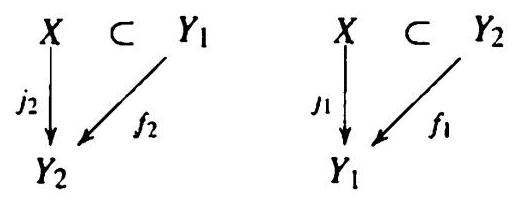
\includegraphics[width=0.4\textwidth]{images/37.3.jpg}
\end{center}
\hspace*{3em} 

The composite \({f}_{1} \circ  {f}_{2} : {Y}_{1} \rightarrow  {Y}_{1}\) has the property that for every \(x \in  X\) , one has \({f}_{1}( {{f}_{2}( x) })  = x\) Therefore, \({f}_{1} \circ  {f}_{2}\) is a continuous extension of the identity map \({i}_{X} : X \rightarrow  X\) . But the identity map of \({Y}_{1}\) is also a continuous extension of \({i}_{X}\) . By uniqueness of extensions (Lemma 38.3), \({f}_{1} \circ  {f}_{2}\) must equal the identity map of \({Y}_{1}\) . Similarly, \({f}_{2} \circ  {f}_{1}\) must equal the identity map of \({Y}_{2}\) Thus \({f}_{1}\) and \({f}_{2}\) are homeomorphisms.
\end{proof}
\begin{definition}
	For each completely regular space \(X\) , let us choose, once and for all, a compactification of \(X\) satisfying the \index{Stone-Čech compactification!extension condition}\index{Stone-Čech compactification!extension condition}\index{Stone-Čech compactification!extension condition}\index{Stone-Čech compactification!extension condition}extension condition of Theorem 38.2. We will denote this compactification of \(X\) by \(\beta ( X)\) and call it the Stone-Čech compactification of \(X\) . It is characterized by the fact that any continuous map \(f : X \rightarrow  C\) of \(X\) into a compact Hausdorff space \(C\) extends uniquely to a continuous map \(g\;\beta ( X)  \rightarrow  C\) .
\end{definition}

\section*{Exercises}
\begin{enumerate}[itemsep=0.4em, parsep=0pt, topsep=0pt, partopsep=0pt, leftmargin=*, label=\arabic*., ref=\arabic*]
\item Verify the statements made in Example 4.
\item Show that the bounded continuous function \(g( {0,1})  \rightarrow  \mathbb{R}\) defined by \(g( x)  =\)  \(\cos ( {1/x})\) cannot be extended to the compactification of Example 3. Define an imbedding \(h : ( {0,1})  \rightarrow  {[  0,1]  }^{3}\) such that the functions \(x,\sin ( {1/x})\) , and \(\cos ( {1/x})\) are all extendable to the compactification induced by \(h\) .
\item Under what conditions does a metrizable space have a metrizable compactification?
\item Let \(Y\) be an arbitrary compactification of \(X\) ; let \(\beta ( X)\) be the Stone-Čech compactification. Show there is a continuous surjective closed map \(g : \beta ( X)  \rightarrow  Y\) that equals the identity on \(X\) [This exercise makes precise what we mean by saying that \(\beta ( X)\) is the ``maximal'' compactification of \(X\) . It shows that every compactification of \(X\) is equivalent to a quotient space of \(\beta ( X)\) .]
\item
  \begin{enumerate}[itemsep=0.2em, parsep=0pt, topsep=0pt, partopsep=0pt, leftmargin=*, label=(\alph*), align=left]
  \item Show that every continuous real-valued function defined on \({S}_{\Omega }\) is ``eventually constant.'' [Hint First prove that for each \(\epsilon\) , there is an element \(\alpha\) of \({S}_{\Omega }\) such that \(| {f( \beta )  - f( \alpha ) }|  < \epsilon\) for all \(\beta  > \alpha\) Then let \(\epsilon  = 1/n\) for \(n \in  {\mathbb{Z}}_{ + }\) and consider the corresponding points \(. {{\alpha }_{n}\text{ . }}]\)

  \item Show that the one-point compactification of \({S}_{\Omega }\) and the Stone-Čech compactification are equivalent.
  \item Conclude that every compactification of \({S}_{\Omega }\) is equivalent to the one-point compactification.
  \end{enumerate}
\item Let \(X\) be completely regular. Show that \(X\) is connected if and only if \(\beta ( X)\) is connected. [Hint: If \(X = A \cup  B\) is a separation of \(X\) , let \(f( x)  = 0\) for \(x \in  A\) and \(f( x)  = 1\) for \(x \in  B\) .]
\item Let \(X\) be a discrete space; consider the space \(\beta ( X)\) .
  \begin{enumerate}[itemsep=0.2em, parsep=0pt, topsep=0pt, partopsep=0pt, leftmargin=*, label=(\alph*), align=left]
  \item Show that if \(A \subset  X\) , then \(\bar{A}\) and \(\overline{X - A}\) are disjoint, where the closures are taken in \(\beta ( X)\) .
  \item Show that if \(U\) is open in \(\beta ( X)\) , then \(\bar{U}\) is open in \(\beta ( X)\) .
  \item Show that \(\beta ( X)\) is totally disconnected.
  \end{enumerate}
\item Show that \(\beta ( {\mathbb{Z}}_{ + })\) has cardinality at least as great as \({I}^{I}\) , where \(I = [  {0,1}]\) . [Hint: The space \({I}^{\prime }\) has a countable dense subset.]
\item
  \begin{enumerate}[itemsep=0.2em, parsep=0pt, topsep=0pt, partopsep=0pt, leftmargin=*, label=(\alph*), align=left]
  \item If \(X\) is normal and \(y\) is a point of \(\beta ( X)  - X\) , show that \(y\) is not the limit of a sequence of points of \(X\) .

  \item Show that if \(X\) is completely regular and noncompact, then \(\beta ( X)\) is not metrizable.
  \end{enumerate}
\item We have constructed a correspondence \(X \rightarrow  \beta ( X)\) that assigns, to each completely regular space, its Stone-Čech compactification. Now let us assign, to each continuous map \(f : X \rightarrow  Y\) of completely regular spaces, the unique continuous map \(\beta ( f)  : \beta ( X)  \rightarrow  \beta ( Y)\) that extends the map \(i \circ  f\) , where \(i : Y \rightarrow  \beta ( Y)\) is the inclusion map. Verify the following:
  \begin{enumerate}[itemsep=0.2em, parsep=0pt, topsep=0pt, partopsep=0pt, leftmargin=*, label=(\alph*), align=left]
  \item If \({1}_{X} : X \rightarrow  X\) is the identity map of \(X\) , then \(\beta ( {1}_{X})\) is the identity map of \(\beta ( X)\) . (ii) If \(f : X \rightarrow  Y\) and \(g : Y \rightarrow  Z\) , then \(\beta ( {g \circ  f})  = \beta ( g)  \circ  \beta ( f)\) . These properties tell us that the correspondence we have constructed is what is called a functor; it is a functor from the ``category'' of completely regular spaces and continuous maps of such spaces, to the ``category'' of compact Hausdorff spaces and continuous maps of such spaces. You will see these properties again in Part II of the book; they are fundamental in algebra and in algebraic topology.
  \end{enumerate}
\end{enumerate}